%%%%%%%%%%%%%%%%%%%%%%%%%%%%%%%%%%%%%%%%%%%%%%%%%%%%%%%%%%%%%%%%%%%%%%%%
\chapter{Introduction}
\label{intro}
%%%%%%%%%%%%%%%%%%%%%%%%%%%%%%%%%%%%%%%%%%%%%%%%%%%%%%%%%%%%%%%%%%%%%%%%
\begin{center}
  \begin{minipage}{0.7\textwidth}
    \begin{small}
      \paragraph{Theodore:} Where are you going?
      \paragraph{Samantha:} It would be hard to explain, but if you ever get there, come find me. Nothing would ever pull us apart. 
    \end{small}
    \begin{flushright}- Her, Spike Jonze (2013) \end{flushright}

  \end{minipage}
\end{center}

Where is Samantha, the artificial intelligence voice system Theodore is in love with, \textit{going}? What is she ``thinking'' about? How is she able to formulate ``thoughts''?

As artificial agents were given some form of intelligence in science-fiction works, the cultural focus has not so much been set on their human (or super-human) abilities, but rather on their frighteningly impenetrable and estranged ``minds''. Mary Shelley's \textit{Frankenstein} famously depicted human fear when faced with a thinking artificial being in the form of the \textit{monster}, a fear that was later framed as the Frankenstein complex by Isaac Asimov in the introduction to his \textit{Robots} series.

Asimov, in turn, presented a paradigm for robotics where the inner reasoning of thinking machines was inhumanly rational, which questioned our ability to align their behavior with the basic goals of humans. Other works have since pushed this paradigm further and presented artificial intelligence (or AI) as an existential threat to humans, as with the murderous HAL9000 computer in Kubrick's \textit{2001: A Space Odyssey}, or even to humankind, as in Frank Herbert's \textit{Dune} series which depicts a galactic war between humans and thinking machines.

Interestingly, as real AI systems grew more and more capable in the past years, especially as they started to excel in mimicking human communication through speech or text, similar fears have been expressed among the general public, and more recently in some parts of the research community. Often framed by its detractors as \textit{AI doomerism}, this school of thought warns about ethical, ecological, social and even security concerns regarding modern systems such as the notorious ChatGPT, framing these models as potential threats to our well-being or even to our existence.

For the layperson, these concerns are based on the mythical statute of AI inherited from the aforementioned cultural representations, coupled with the current lack of general education regarding machine learning. For the initiated, these concerns are scientifically rooted in the fact that modern AI models are \textit{non-symbolic}, which implies that their inner workings have been automatically optimized to match a desired behavior, rather than handcrafted on the basis of expert knowledge. As such, understanding these inner workings can only be done \textit{a posteriori}, and is often particularly hard, especially in the context of text-based AI systems. This has led to a common depiction of modern AI systems as \textit{black-box} models, which leads to a scientific transposition of the Frankenstein effect.

Nevertheless, these concerns have been expressed against the current tide of impressive acceleration of both quantifiable and perceived capabilities of artificial intelligent systems, which can be explained by the success of what we shall call the \textit{behaviorist} approach.

\section{Artificial Behaviorism}

In psychology, behaviorism is a school of thought that flourished in the first half of the 20\up{th} century. It can be traced back to the works of Edward Thorndike and Ivan Pavlov on \textit{reinforcement}, that prove that some reflexes and actions of a human or animal being can be progressively shaped by the consistent application of positive or negative consequences responding to its behavior. 

In 1924, this theory was extended by John B. Watson who introduced \textit{methodological} behaviorism, a model of observed behavior that rejects introspection and is based solely on stimuli and environment. B.F. Skinner later framed cognition itself as a behavior that can be explained by stimuli and environment.

Overall, behaviorists frame the study of minds as an input-output analysis of agents, and argue that explaining a response based on an environment and immediate stimuli, which include a reinforcement history and an internal state of the subject. One of the main limitation of this framing is the difficulty to explain the observation of behaviors that cannot be entirely explained by conditioning and reinforcement, such as the ability to produce novelty, especially observed in language.

The more recent \textit{cognitive} psychology theory takes a radically different stance and thoroughly models minds as a combination of complex specialized subsystems that interact with each other, in an attempt to provide explanations to the observed novelty and generalization abilities of biological beings.

In computer science, the recent advances regarding intelligent systems that handle text, images and sound have led to the emergence of technologies that display anthropomorphic abilities, often leading to users (and even inventors) referring to these technologies as actual beings \citep{anthropo}. The anthropomorphization of AI models can be linked to the Turing test \citep{turing1950computing}, a thought experiment that quantifies the intelligence of an artificial agent capable of generating text, by measuring the amount of human testers that fail to identify this agent as non-human, the testers being informed of the nature of the test. More modern evaluation approaches consist in building lists of tasks that are designed to measure intelligence on the basis of a given criterion, and in analyzing the performance of a model based on its ability to correctly solve the tasks.

These technologies rely on highly parameterized statistical models that can approximate a wide range of input-output mappings or \textit{functions} \citep{HORNIK1990551}. The parameters of these models are then optimized in a way that reduces the discrepancy between the model's output and the expected result. In \textit{self-supervised} approaches, these models learn to approximate functions that correspond to raw data, e.g. that maps a truncated text segment as an input to the next truncated word as an output.

Hence, \textbf{the modern approach to designing artificial agents is deeply connected to a behaviorist view of cognition}, both in its final purpose and in the means it uses to reach this purpose. As a matter of fact, the Turing test, as well as current evaluation benchmarks, are behaviorist by nature, as they measure the ability of an artificial agent to produce a desired reaction to a given input. Moreover, the optimization procedure, or \textit{training}, of the parameterized models resembles the reinforcement phenomenon documented in the first works of behaviorists.

\begin{figure}[ht]
  \centering
  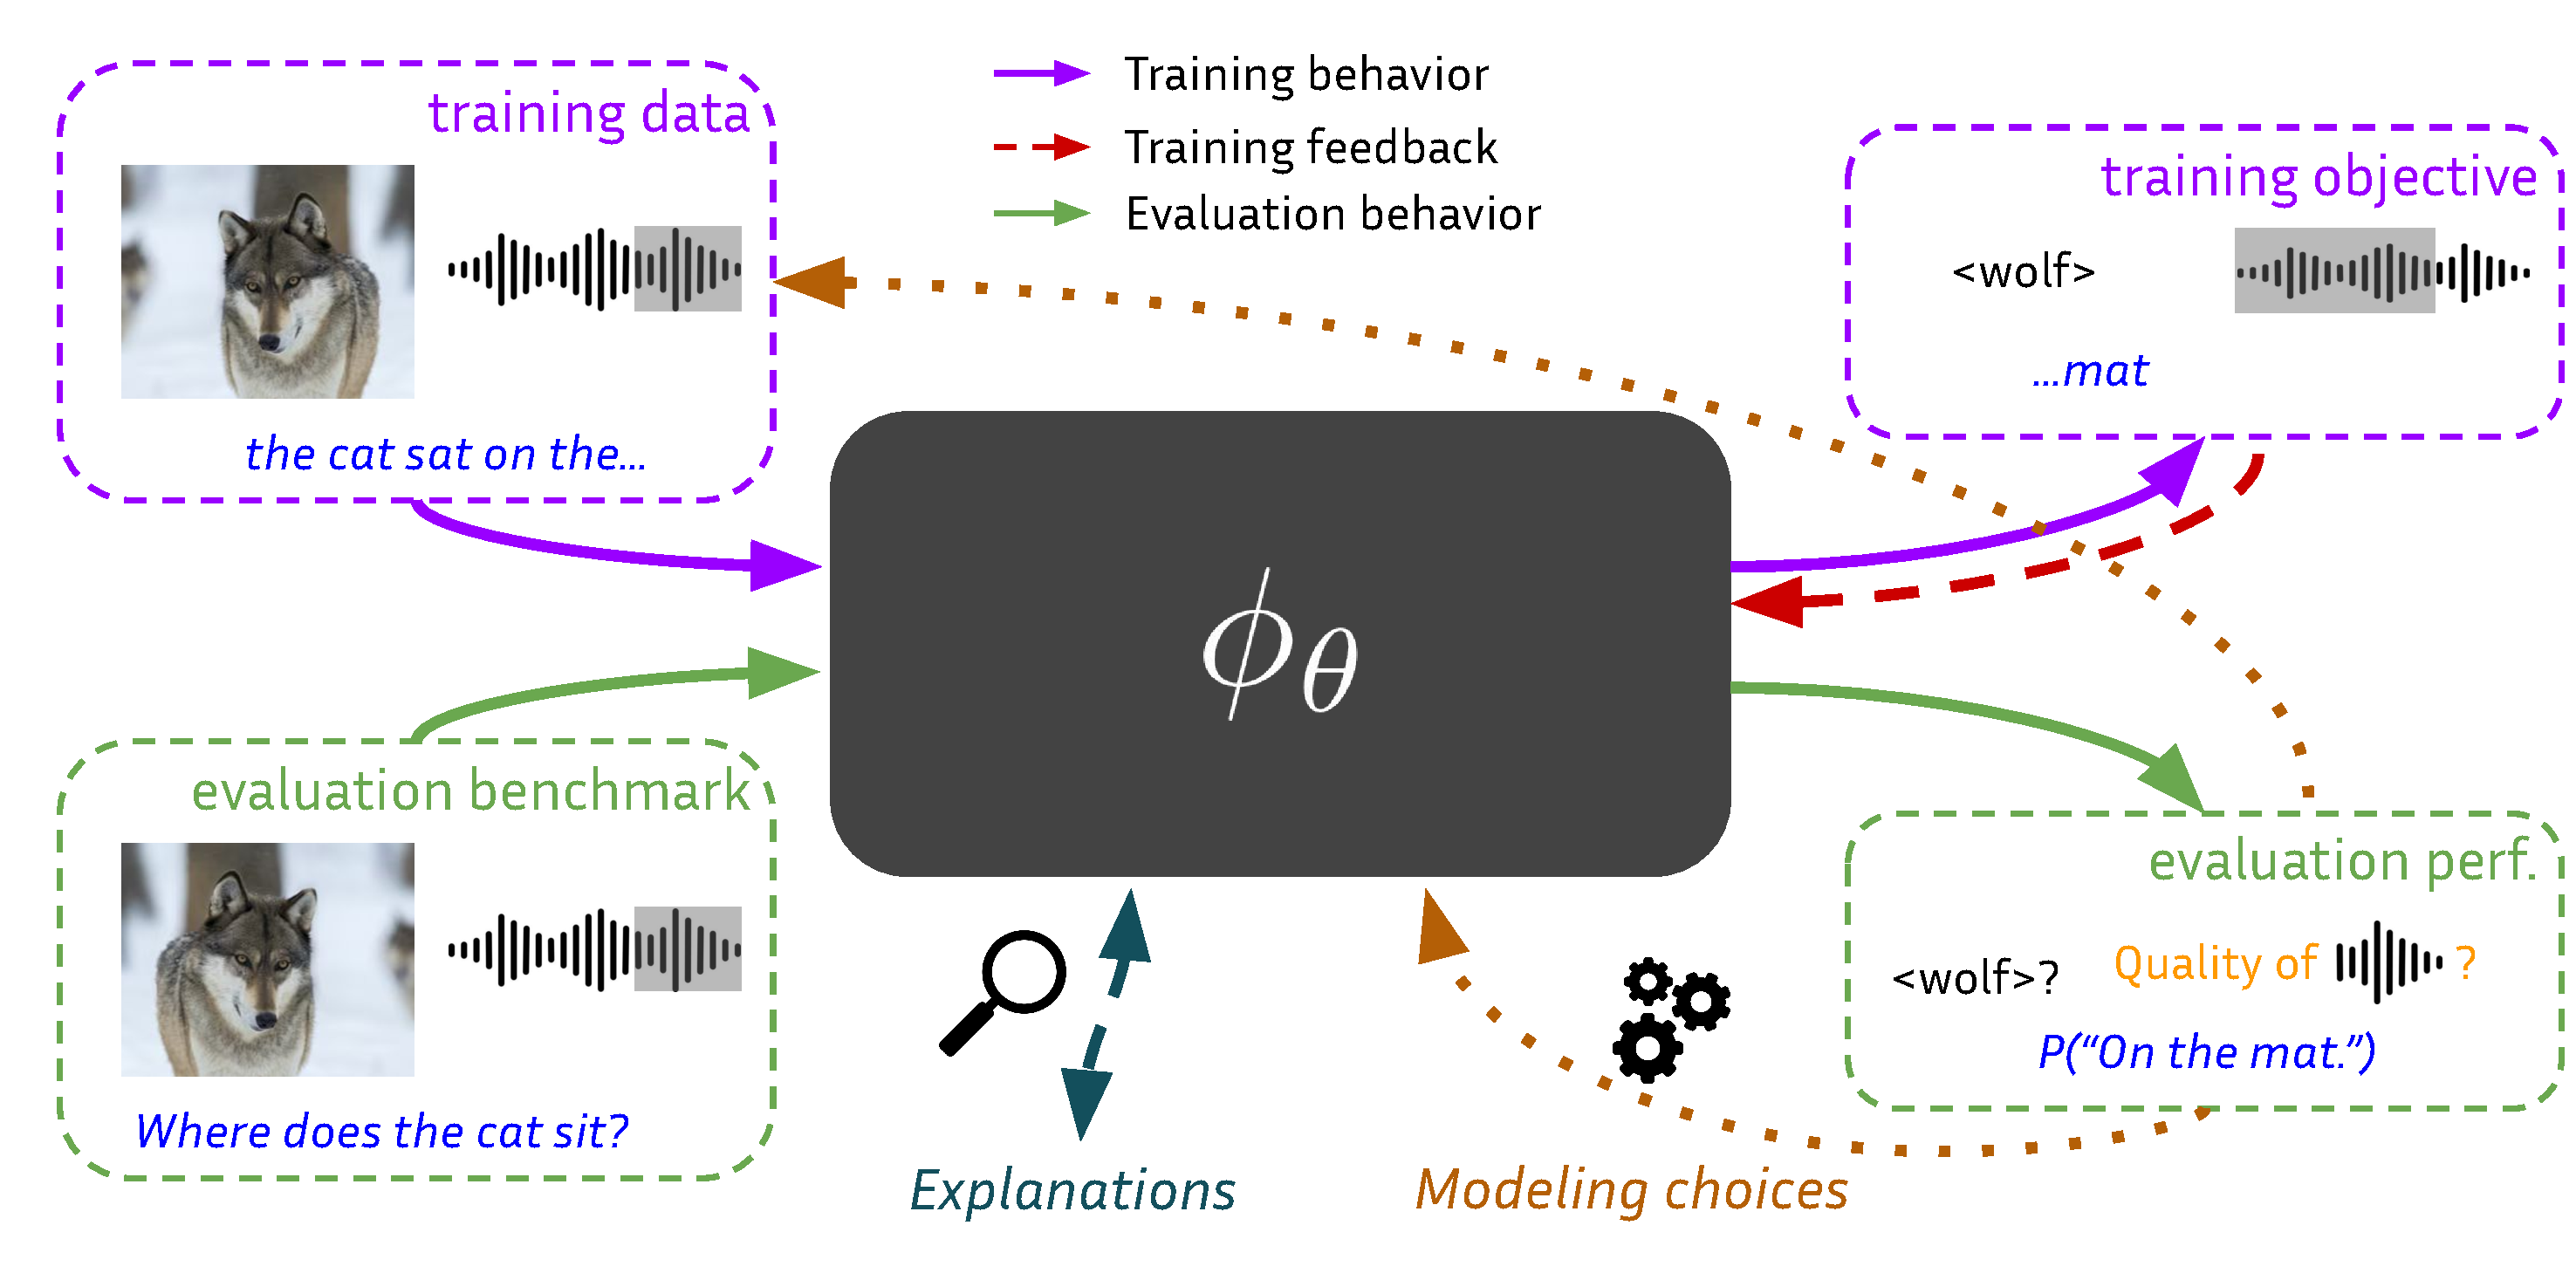
\includegraphics[width=0.9\linewidth]{sources/imgs/behaviorist_schema.pdf}
  \caption{Schematic overview of the behaviorist paradigm in AI.}
  \label{fig:behaviorist}
\end{figure}

As pictured in \Cref{fig:behaviorist}, this paradigm directs design choices, such as the inductive biases that are implemented in the models, i.e. the architectural decisions that are made with respect to their inner workings, the data used for training, or the details of the optimization process. These choices are guided by the ability of resulting models to extensively capture reinforcement feedback during training, and by their ability to correctly display an expected ``intelligent'' behavior during evaluation. Over the past years, such artificial behaviorism has been widely pushed forward by industrial actors, because of its impressive ability to achieve what it was designed for, that is, produce human-like responses to users' stimuli and real-world environments. 

The rising interest for such technologies has also raised a will to explain and interpret the behaviors of resulting models using post-hoc methods. Even though these methods propose to dissect the models' internal patterns, they are also framed in a behaviorist way, as they are aimed at answering the question of behavior at a smaller scale, namely \textit{how will each part of the model behave when faced with this given input?}

More recent developments in the field of text-based AI, or \textit{language models}, have further illustrated the extent of the behaviorist approach. A line-of-work has consisted in representing these models as highly-evolved compression schemes for training data \citep{huang2024compression,deletang2024language}, which is a view that stresses out the inherent importance of a certain proximity between the reinforcement signals and the evaluation stimuli. A different line-of-work has promoted the use of \textit{chain-of-thought} writing style in the generated responses of language models \citep{wei2022chain}, based on the hypothesis that the reasoning explanation itself is a useful signal that helps to produce the correct final response. This is intrinsically based on a strongly behaviorist view of reasoning, as it displaces the reasoning mechanisms from the inner transformations of the models to the input-output space, allowing the model to use its own output as a stimulus.

The behaviorist paradigm has brought remarkable capabilities to AI systems under its own evaluation criteria, but also from a productivity-oriented technological point of view, as many tasks can be automated using these systems. Nevertheless, it is both unsure that these models will be able to reach \textit{general} intelligence, and that the behaviorist framework itself is sufficient to quantify general intelligence, or even define it. In other words, it is far from certain whether both training and evaluating models as pure input-output mappings will be sufficient to reach ``human-like'' intelligence, as one of the founders of modern AI himself has stated \citep{lecun2022path}.

\section{Limitations of Modern Approaches}

It could be argued that the behaviorist approach is conceptually limited by its inability to properly assess intermediate states of cognition. For instance, behaviorist evaluation will favor a model that makes predictions based on spurious correlations, such as identifying a wolf in an image based on the white background that evokes snow \citep{10.1145/2939672.2939778}, to a model that would internally be able to properly represent the concept of ``wolf'', by mapping it internally to a specific geographical zone, a sound, or other related concepts, but that would be unable to produce the expected output. The existence of such a model is even absurd under the behaviorist paradigm, because the intrinsic ability of the model to map relevant concepts together would be conditioned by its ability to provide the right answer. This limitation, among other reasons, has motivated \textit{neuro-symbolic} methods in recent years \citep{10148662}.

However, beyond conceptual limitations that we shall not elaborate here, the current approach to AI systems and more particularly language models is faced with limitations, both from the technical and scientific view points.

Self-supervised learning has empirically been shown to yield more performant models as the number of relevant training samples increased. Over the years, engineers and researchers working on language models have extensively gathered web-crawled data through various initiatives such as Common Crawl, that led to the creation of several filtered data resources \citep{oscar,gao2020pile,penedo2024finewebdatasetsdecantingweb}. Yet, even the trillions of words that are available on the internet are not sufficient to exhaustively cover the possibilities of natural language, and it is not guaranteed that it will be possible to obtain significantly more textual relevant data in the near future.

Moreover, it was recently shown that increasing the amount of parameters used in the neural architectures that constitute language models systematically led to better performance for similar training data, contrarily to the belief that larger models would over-fit, i.e. perfectly approximate training data at the expense of generalization capabilities. Nevertheless, these larger models pose major technical challenges in terms of hardware efficiency and requirements, both during training and when the models are used at \textit{inference} time. These physical constraints in turn yield energetic, ecological and economical concerns, as these more demanding models lead to more intensive power consumption, to the extraction of more raw material to build the processing units, and to the use of more costly computation infrastructure \citep{ecolo_llm}.

Evaluation benchmarks have been prone to saturation, as models reached performance levels that did not allow to significantly distinguish them from one another based on their scores on these benchmarks. This can be explained by the ever-growing training data coverage that inevitably includes examples that help with the specific task at hand, and by the increasing size of models that allows to better memorize these examples. This raises concerns about explicit or implicit contamination, i.e. the presence of evaluation data or a variation thereof in the training dataset, but also about an implicit optimization of the training data mix to optimize the downstream performance on these benchmarks, at the potential expense of generalization abilities. As such, new benchmarks are often designed with fresh data in order to avoid as much as possible these risks, and to try to evaluate the truly \textit{zero-shot} abilities of the language models.

Finally, the behaviorist view raises challenges when the relevance of a response is harder to evaluate, which may happen in machine translation, but also when assessing models from a security and ethical point of view, in what is referred to as \textit{model alignment}. In that field, the responses of language models are themselves viewed as complex text utterances, and it is harder to tell whether a model has responded correctly to a malicious stimulus. Moreover, there is no guarantee that models will never produce harmful content at inference time, as the variation of stimuli that can be produced by users cannot be anticipated exhaustively.


\section{Motivations}

The behaviorist approach has undeniably led to major advances in the field of artificial intelligence, and more noticeably in the language modeling domain over the recent months. Yet, it is meeting significant challenges that raise deep scientific, engineering, and even philosophical questions.

\begin{figure}[ht]
  \centering
  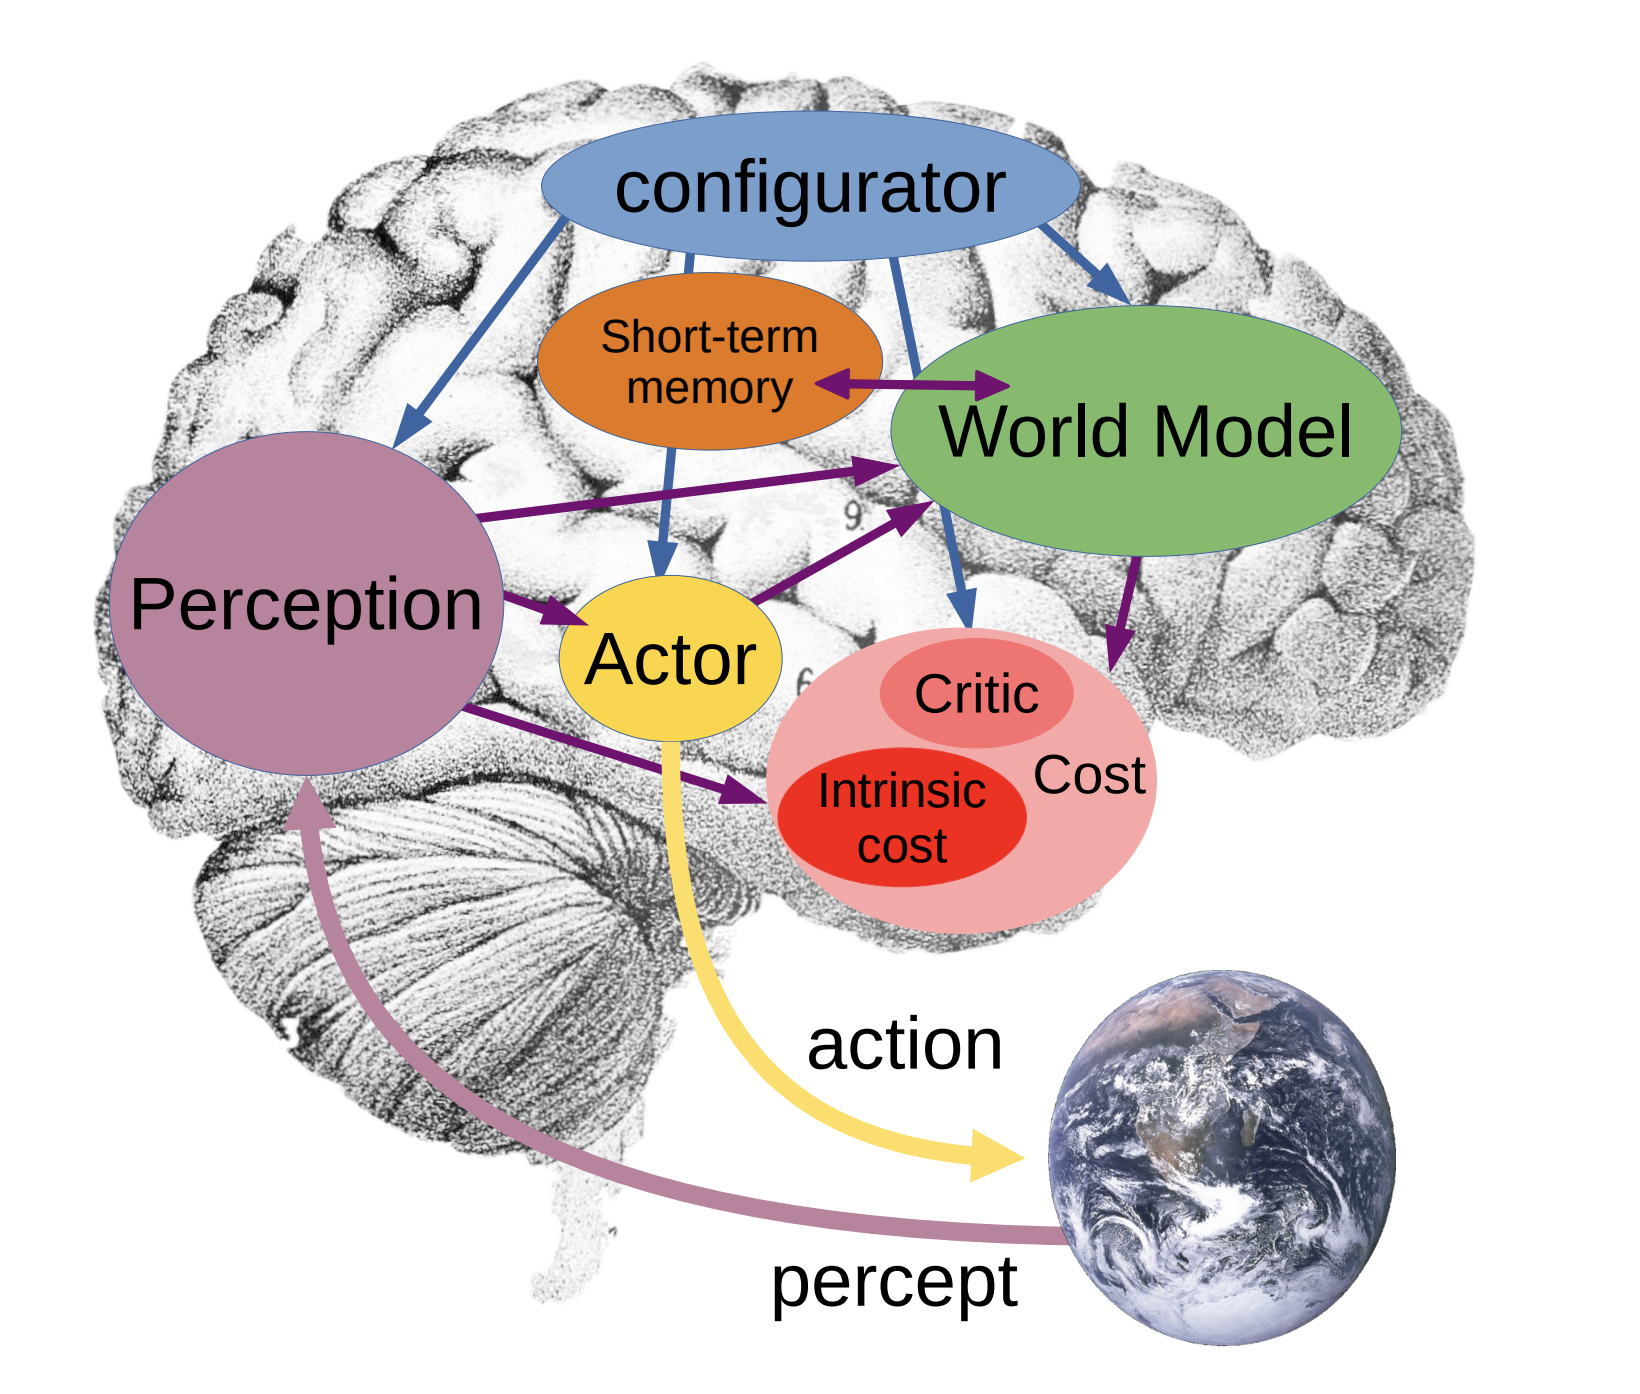
\includegraphics[width=0.5\linewidth]{sources/imgs/jepa_arch.png}
  \caption{The cognitive architecture presented in \citet{lecun2022path}.}
  \label{fig:lecun_jepa}
\end{figure}

Does that mean that we should build a completely new paradigm for machine learning? This is what Yann LeCun has advocated in the last few years, notably with his \textit{Joint Embedding Predictive Architecture} \citep{lecun2022path}, that designs a model for artificial ``minds'' based on several specialized subsystems that interact with each other (see \Cref{fig:lecun_jepa}). This work could be framed as a transposition of cognitive psychology to artificial intelligence, with the exception that the former devises a model of a functional system that itself defines what we call human intelligence, namely the human mind, while the latter proposes to mimic this potentially imperfect model of the human mind in artificial systems, in the hope to reach a similar intelligence level. It can be opposed to this approach that using an explanatory model of the mind to build a functional system that should reach human performance amounts to considering that this model exhaustively captures the complexity of the human mind, which is not certain. Hence, handcrafting such a model of cognition is a subjective and very empirical approach to artificial intelligence and is not guaranteed to work.

\vspace{1em}

We argue that if a transition similar to the one from behaviorism to cognitive psychology should operate in machine learning, it should first focus on how we \textit{evaluate} AI models rather than on how we design them. In other words, we should aim at building models that could be analyzed \textit{a posteriori} in a way that resembles how cognitive psychology analyzes human cognition, even when those models were not \textit{a priori} designed to mimic an explanatory model of cognition. Evaluating models through their ability to exhibit internal behaviors that mimic human cognition, or through the ease with which they can inherently learn desired cognitive patterns, may provide insights that in turn lead to better model design.

One way to initiate this work is to dissect the inner workings of the models that follow the behaviorist framework, and to observe in a quantitative and qualitative way their ability to manipulate representations of concepts and items they are implicitly required to handle to solve the task they are designed for. Interestingly, significant recent advances in the field of language modeling have implicitly taken a similar stance. The well-known Transformer work \citep{vaswani2017attention} started from the observation that the previous recurrent counterparts failed to correctly model long-range interaction. Low-rank adaptation of language models \citep{hu2022lora} was made possible by empirical observations on the structure of the parameters in language models. More recently, lossless generation acceleration was allowed by the analysis of attention sinks in the inner patterns of language models \citep{xiao2024efficient}.

In this work, we specifically focus on text-based AI, i.e. language modeling in its modern form, and we apply the aforementioned philosophy to analyze the representational spaces of language models in view of stretching their limitations. We summarize our research questions in the following points:

\begin{itemize}
  \item What can we learn if we look at language models in a non-behaviorist way? Can an analysis of the inner representations of these models yield conclusions that question the current paradigm?
  \item Beyond caveats, can we identify bottlenecks and seemingly suboptimal mechanical inner workings if we look beyond the input/output efficiency of classical approaches?
  \item Can we design methods that alleviate models from these bottlenecks and lead to improvements in language modeling?
\end{itemize}

\section{Contributions}

We begin our work by a thorough analysis of the inner workings of language models, that employs a mechanical view of their architectures from several viewpoints throughout \Cref{part:analysis}.

In \Cref{chap:geobias}, we empirically measure their ability to represent real-world concepts with the example of geographical bias, and the relation between this ability and the scaling philosophy of recent advances in the field. Our observations confirm the positive impact of scale on performance as framed in a behaviorist way, but we identify a negative impact of scale on the intrinsic ability of language models to improve their inner representations independently of the imbalanced data distribution, even showing that larger models tend to augment this frequency-based bias. 

We proceed to further analyze the impact of textual data distributions on the representations of language models from a general geometrical perspective in \Cref{chap:softmax_bottleneck}. We identify a general bottleneck in language models in the transition from compact output representations to word-level probability distributions. We correlate this bottleneck with both a degeneration phenomenon, where the representational spaces of models collapse, and a performance saturation during training that affects smaller language models.

In \Cref{chap:anisotropy}, we notice that this geometrical degeneration phenomenon affects deeper inner representations of the models, and we propose to explain this phenomenon from the perspective of the inductive biases commonly used in modern models, namely self-attention layers. We link this intrinsic degeneration to the \textit{sparsity} of the attention mechanisms in language models, arguing that the need for sparsity imposes such distortions to the underlying latent spaces.

We proceed to research solutions to some of the aforementioned limitations in \Cref{part:analysis}. 

\Cref{chap:headless_lm} introduces a training objective that mitigates frequency-based distortions and reduces the geometrical effect of the prediction layer of language models described in \Cref{chap:softmax_bottleneck}. Incidentally, this method substantially improves the efficiency of training for a wide range of models from several viewpoints.

We proceed by attempting to further mitigate representation degeneration by modifying the granularity of the predicted textual units in \Cref{chap:manta}. Although our efficient gradient-based text segmentation method improves the robustness of language models to noisy text utterances, and occasionally boosts their performance, it fails to mitigate the inner degeneration effects described in \Cref{chap:anisotropy}.

Thus, we finally propose a framework in \Cref{chap:kv_comp}, that provides a path towards denser self-attention maps, in the hope to mitigate the distortions observed in \Cref{chap:anisotropy}, and to improve model efficiency and scalability in the process.

The work presented in this thesis has led to several publications in international natural language processing (NLP) and machine learning (ML) conferences:
\begin{itemize}
    \item \textit{MANTa: Efficient Gradient-Based Tokenization for Robust End-to-End Language Modeling}, presented at EMNLP 2022, and co-authored by Roman Castagné;
    \item \textit{Is Anisotropy Inherent to Transformers?}, presented in the Student Research Worskhop at ACL 2023;
    \item \textit{Anisotropy Is Inherent to Self-Attention in Transformers}, presented at EACL 2024;
    \item \textit{On the Scaling Laws of Geographical Representation in Language Models}, presented at LREC-COLING 2024;
    \item \textit{Headless Language Models: Learning without Predicting with Contrastive Weight Tying}, presented at ICLR 2024;
    \item \textit{Why do small language models underperform? Studying Language Model Saturation via the Softmax Bottleneck}, presented at COLM 2024.
\end{itemize}